\documentclass{SBCbookchapter}
\usepackage{graphicx}
\graphicspath{{figures/}}
\usepackage[utf8]{inputenc}
\usepackage[T1]{fontenc}
\usepackage[brazil,english]{babel}
\usepackage{array}
\usepackage{setspace}
\usepackage{colortbl}
\usepackage{listings}
\usepackage{amsmath}
\usepackage[hyphens]{url}
\usepackage{setspace}
\usepackage{amssymb}
\usepackage[font=small,labelfont=bf]{caption}
\usepackage{fancyhdr}
\usepackage{pdfpages}
\usepackage{xcolor}
\usepackage{tabularx}
\usepackage{tocloft}
\usepackage[
backend=bibtex,
style=apa,
sorting=ynt
]{biblatex}

\addbibresource{references.bib}

\addtolength{\cftsecnumwidth}{10pt}
\addtolength{\cftsubsecnumwidth}{10pt}


% Set up colour scheme for code blocks

\definecolor{codegreen}{rgb}{0,0.6,0}
\definecolor{codegray}{rgb}{0.5,0.5,0.5}
\definecolor{codepurple}{rgb}{0.58,0,0.82}
\definecolor{backcolour}{rgb}{1,1,1}

\setlength{\tabcolsep}{20pt}

\lstdefinestyle{inlinestyle}{
    backgroundcolor=\color{backcolour},   
    commentstyle=\color{codegreen},
    keywordstyle=\color{magenta},
    numberstyle=\color{codegray},
    stringstyle=\color{codepurple},
    basicstyle=\ttfamily,
    breakatwhitespace=false,         
    breaklines=true,                 
    captionpos=b,                    
    keepspaces=true,                 
    numbers=left,                    
    numbersep=5pt,                  
    showspaces=false,                
    showstringspaces=false,
    showtabs=false,                  
    tabsize=2
}

\lstdefinestyle{mystyle}{
    backgroundcolor=\color{backcolour},   
    commentstyle=\scriptsize\color{codegreen},
    keywordstyle=\color{magenta},
    numberstyle=\tiny\color{codegray},
    stringstyle=\scriptsize\color{codepurple},
    basicstyle=\ttfamily\scriptsize,
    breakatwhitespace=false,         
    breaklines=true,                 
    captionpos=b,                    
    keepspaces=true,                 
    numbers=left,                    
    numbersep=5pt,                  
    showspaces=false,                
    showstringspaces=false,
    showtabs=false,                  
    tabsize=2
}

% Add functions so that they are properly highlighted in code blocks

\lstdefinelanguage{tidyqpcr}
{morekeywords={aaa, display_plate_value, calculate_efficiency_bytargetid,calculate_deltacq_bysampleid,calculate_deltadeltacq_bytargetid,calculate_normvalue,create_blank_plate,label_plate_rowcol,create_colkey_4diln_2ctrl_in_24,create_rowkey_4_in_16,read_lightcycler_1colour_raw,calculate_drdt_plate,factor,rep,paste0,create_colkey_6_in_24,system.file,read_lightcycler_1colour_cq,left_join,mutate,bind_rows,unite,tibble,filter,group_by,summarize,median,ggplot,geom_point,aes,position_jitter,facet_wrap,scale_y_log10,label_number,theme,element_text,function,assert_that,has_name,pull,norm_function}
sensitive=false,
morecomment=[l]#,
morestring=[b]"}
\lstset{style=inlinestyle, language=tidyqpcr}

\usepackage{blindtext}

\usepackage{subfiles} % Best loaded last in the preamble

\setcounter{secnumdepth}{-1}

% add chapter titles to toc
\renewcommand{\cftchapfont}{\bfseries}
\renewcommand{\cftchappagefont}{\bfseries}
\renewcommand{\cftchappresnum}{Chapter }
\renewcommand{\cftchapaftersnum}{:}
\renewcommand{\cftchapnumwidth}{6em}

\begin{document}
\title{Developing Open-Source Analysis Software for the Quantification of RNA Transcript Abundance}
\author{Samuel Joseph Haynes}
\date{2022}
\makethesistitle

\newpage

\renewcommand{\thepage}{\roman{page}}

\chapter{Dedication}

%To Wayne, Angela, Charlotte, and all the fools who call me friend.

\newpage

\chapter{Declaration}
I declare that this thesis was composed by myself, that the work contained herein
is my own except where explicitly stated otherwise in the text, and that this work has
not been submitted for any other degree or professional qualification.

Samuel Haynes 
2022

\newpage

\chapter{Acknowledgements}

\newpage

\chapter{Abstract}

%\subfile{chapters/abstract}

\newpage

\chapter{Lay Summary}

\newpage

\tableofcontents

\newpage

\listoffigures

\newpage

\listoftables

\newpage

\pagestyle{fancy}
\fancyhf{}
\fancyhead[RO]{\nouppercase{\rightmark\hfill\thepage}}
\fancyhead[LE]{\nouppercase{\thepage\hfill}}

\renewcommand{\thepage}{\arabic{page}}

\setcounter{page}{1}
\setcounter{chapter}{0}

\setcounter{secnumdepth}{3}

%\chapter{Introduction}

\subfile{chapters/introduction}

\newpage

\subfile{chapters/materials_and_methods}

\newpage

%\chapter{tidyqpcr}

\subfile{chapters/tidyqpcr_chapter}
\newpage

\subfile{chapters/chimera_chapter}
\newpage

\subfile{chapters/differential_fractionation_chapter}

\newpage

\subfile{chapters/discussion_chapter}

\newpage

\setcounter{secnumdepth}{-1}

\printbibliography[heading=bibintoc]

\newpage

\chapter{Appendix}

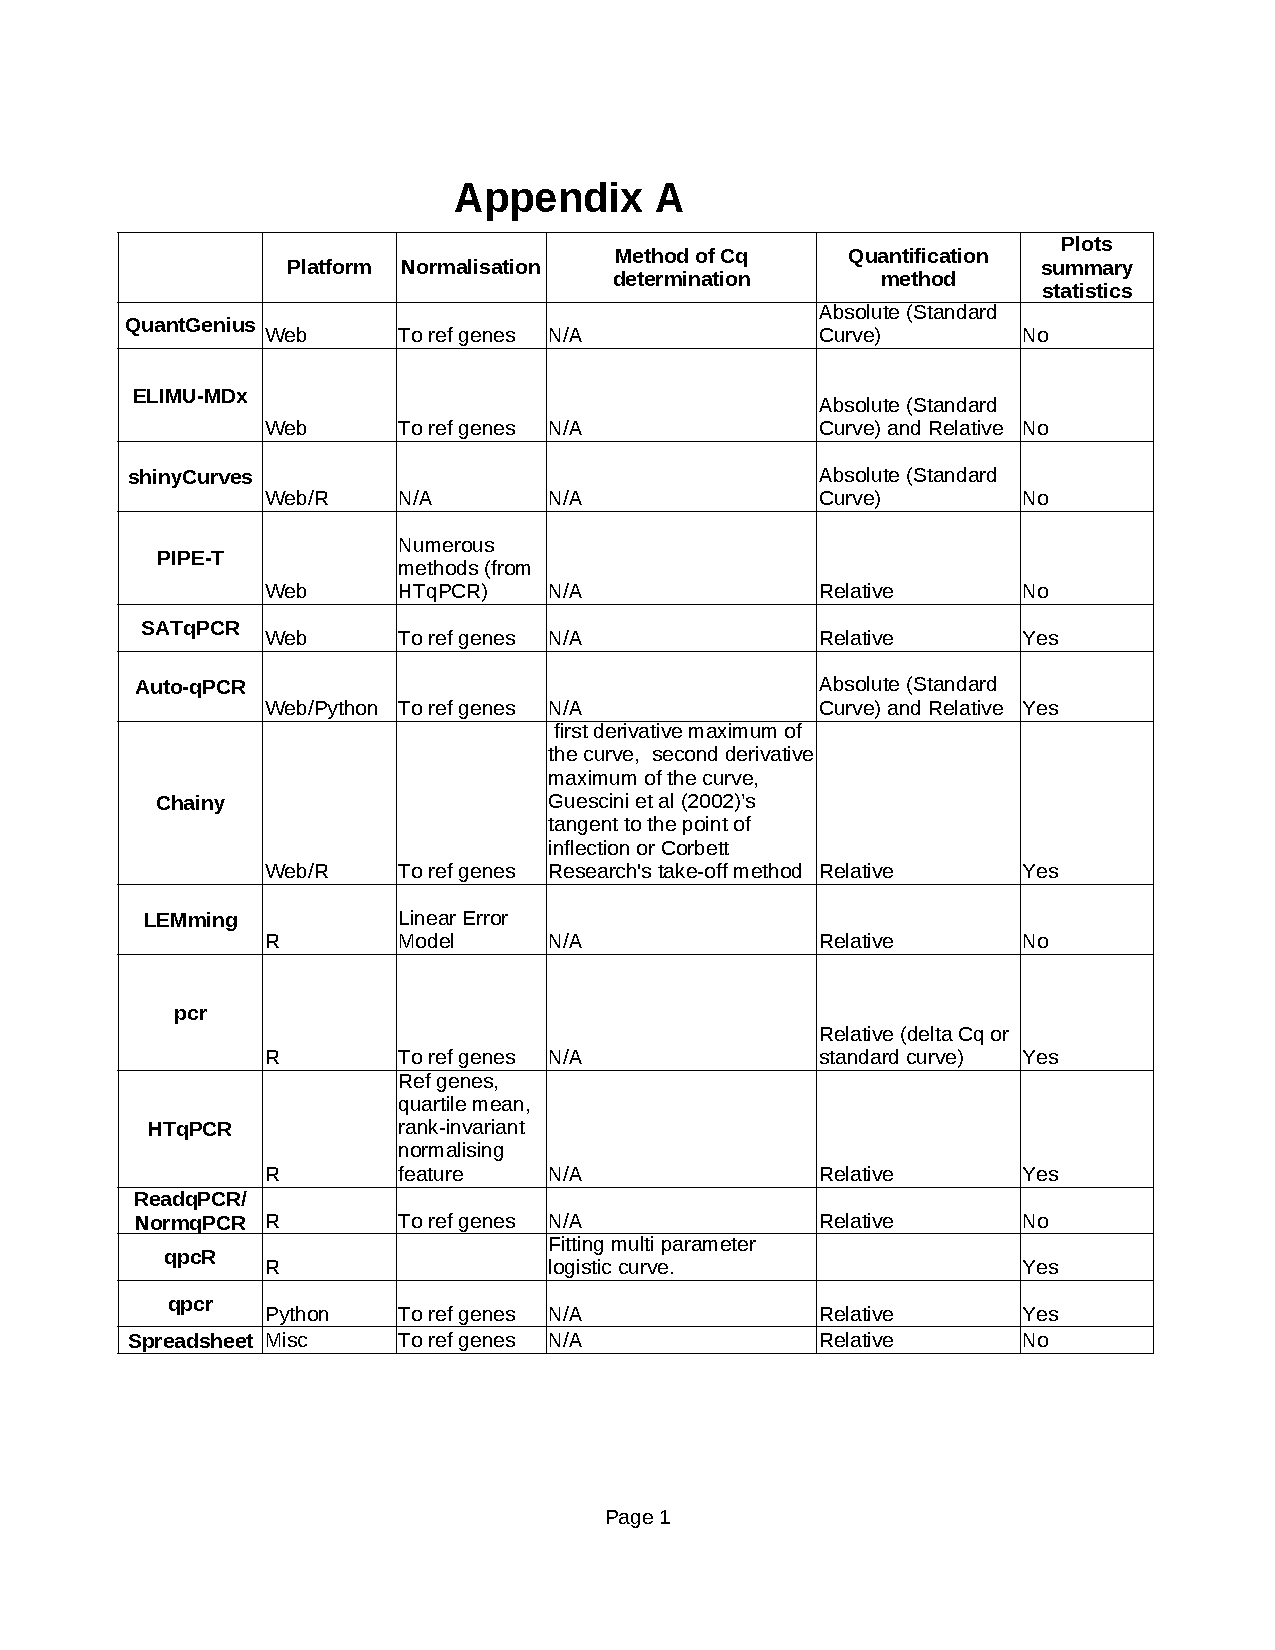
\includepdf[pages=1-4]{chapters/tidyqpcr_appendix_A}

\newpage

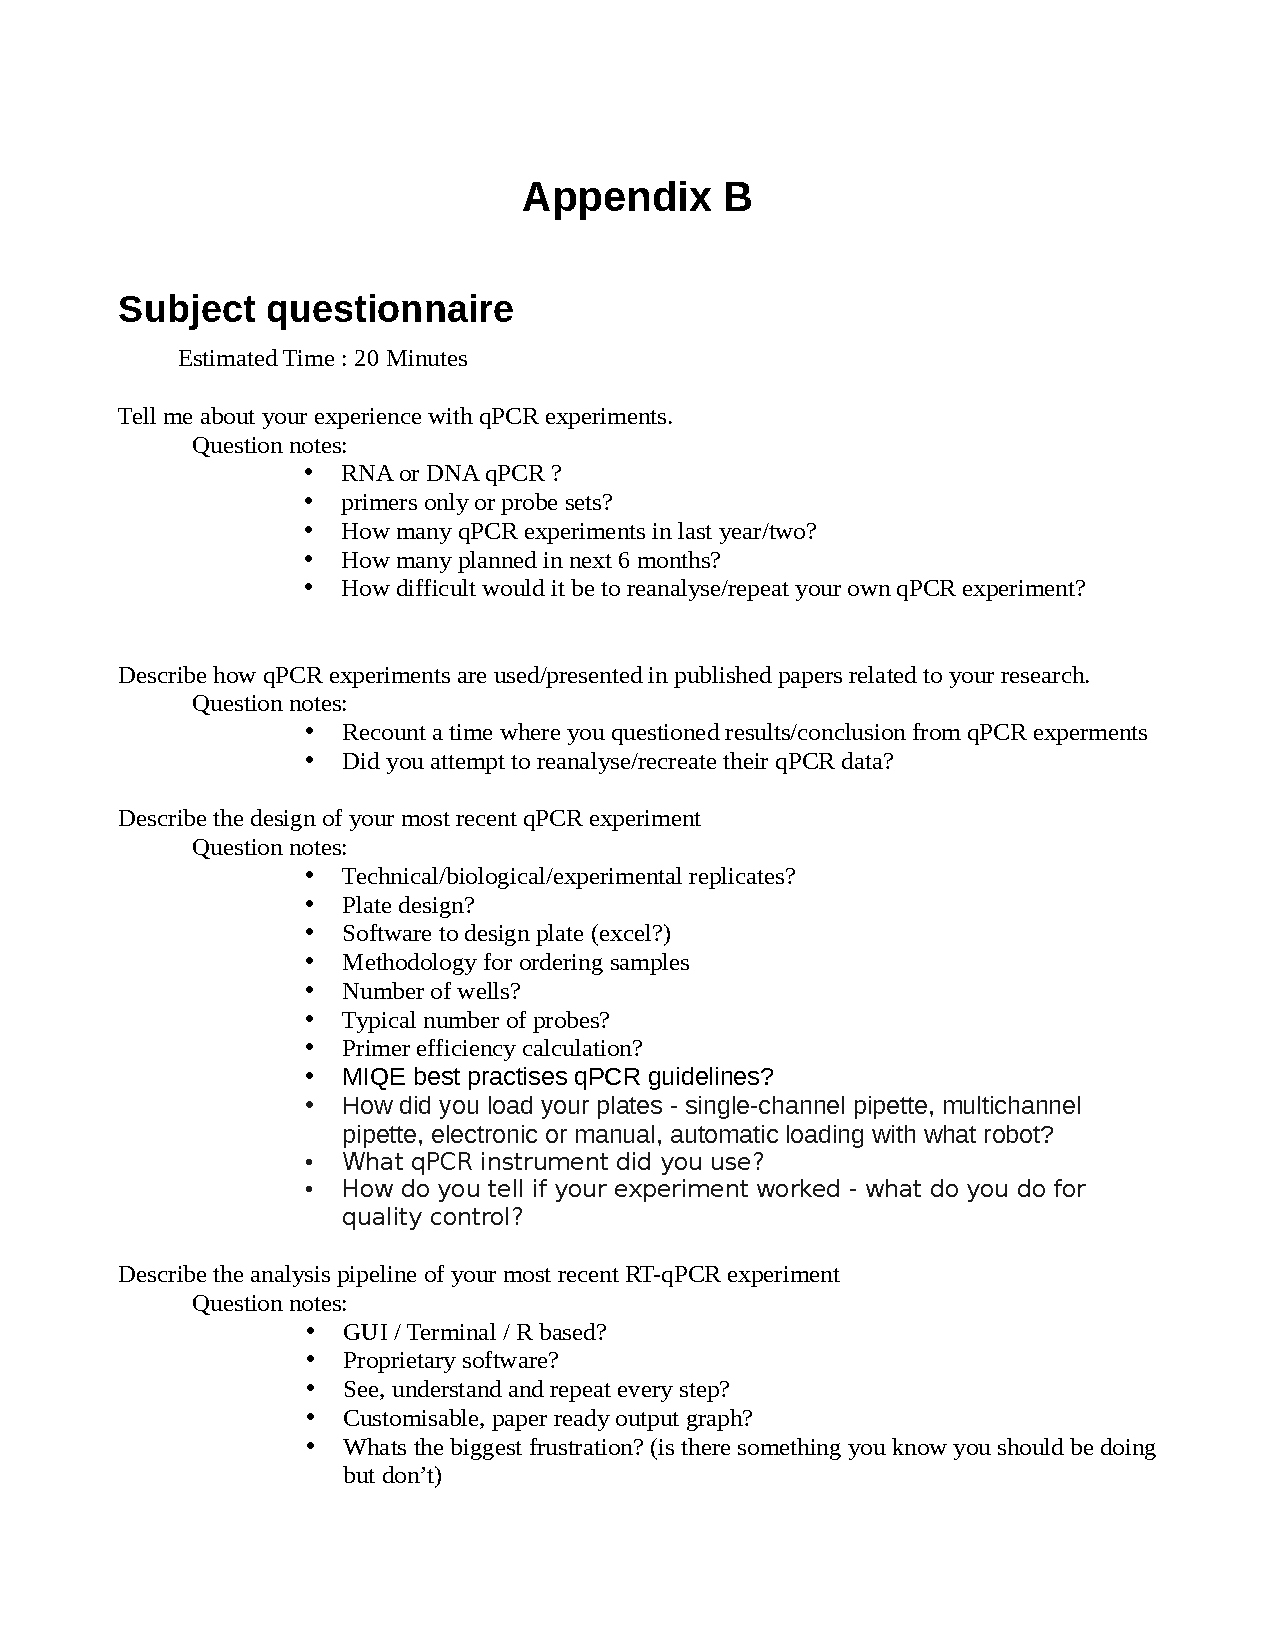
\includepdf[pages=1-2]{chapters/tidyqpcr_appendix_B}

\newpage

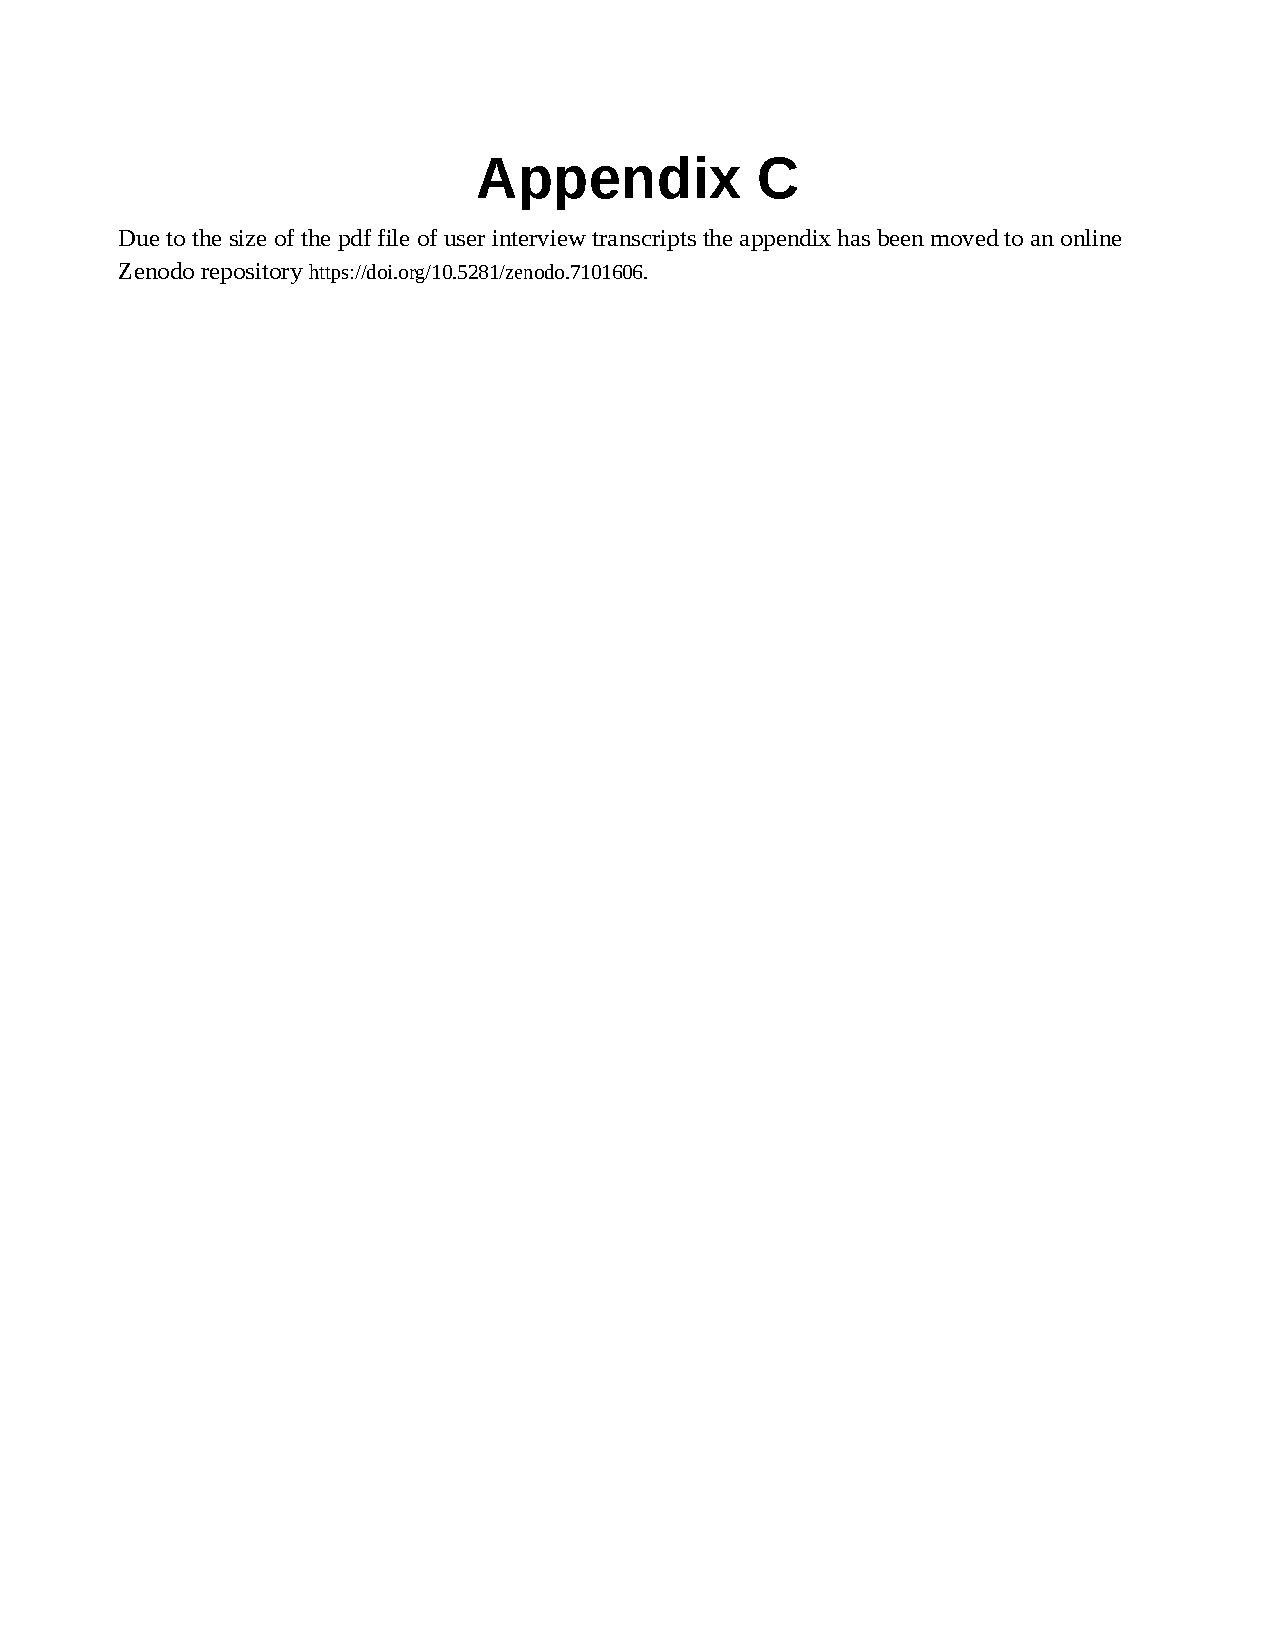
\includepdf{chapters/tidyqpcr_appendix_C}

\newpage

\subfile{chapters/chimera_chapter_supp_data}

\end{document}